\chapter{Range queries in the persistent model}
\thispagestyle{myheadings}

	There are plenty of works offering range query solutions in a snapshot adversary model.
	Some authors propose a new \acrfull{ore} scheme to be used inside an existing range query index, see \cite{bclo-ope,clww-ore,lewi-wu-ore,cloz-ore,fh-ope}.
	Others suggest complete client-server protocols with different security guarantees, see \cite{florian-protocol,pope,practical-ore}.

	Instead of adding another solution to the mix, we developed a robust evaluation framework to compare and audit different \acrshort{ore} schemes and range query protocols \cite{ore-benchmark-17}.
	We have noticed that all proposed solutions offer their own formal protocol, security definition (which they obliviously satisfy), and even performance metrics.
	Moreover, only a few of these algorithms have ready-to-use open-sourced code.
	More often, the implementation is a prototype (or does not even exist), rendering experiments non-reproducible.

	Our work addresses these shortcomings.
	We proposed a common framework where all analyzed solutions follow the same formal protocol, a variant of an outsourced database from \cref{section:proposal:intro:model}.
	The schemes and protocols are also tested against the same security definition, a variant of a simulation-based security game where the simulator has a leakage function that is different for each solution.
	Lastly, all protocols are implemented in the same language and runtime, and are using the same cryptographic primitive implementations.

	We have paid extra attention to how we quantify the performance.
	Published works typically claim that they have implemented the algorithm in some language and ran it on a server many times measuring the wall-clock time.
	Such metric is deeply flawed since it only measures just that --- the wall-clock time it took for a particular machine to execute a particular code that references particular implementations of primitives and makes (or even does not make) \acrshort{io} requests to particular hardware.
	What we offer is a metric that drops all these ``particulars'' (i.e., dependencies) from the protocol execution.
	On top of having all solutions implemented in the same language and using the same primitives, instead of measuring the time we count the number of times an \acrshort{ore} scheme makes use of a primitive and a protocol makes an \acrshort{io} request.
	This metric is much more demonstrative: one can always get a wall-clock time estimate given these counts and the specs of the hardware.
	Moreover, we can analyze these counts theoretically from the pseudocode and then verify them practically after running the code.

	\section{\acrshort{ope} and \acrshort{ore} schemes}

		One of the ways to run a range query in the presence of a snapshot adversary is to use a conventional database range index, such as \BPlus{} tree~\cite{b-tree}, and encrypt the values in the index in a way that preserves their comparison result.
		This is exactly what \gls{ope} does.
		\gls{ope} is a scheme, a tuple of algorithms \algo{OPE.KeyGen}, \algo{OPE.Enc} and \algo{OPE.Dec}, that generate a kay, encrypt and decrypt a number respectively with a property that if $x$ was smaller, greater or equal to $y$, then their respective ciphertexts will maintain the relation.
		\gls{ore} works similarly except that the ciphertexts are not necessarily numbers and a comparison is an explicit algorithm \algo{ORE.Cmp} over hte ciphertexts.
		Formally, \gls{ope} is a specific \gls{ore} where ciphertexts are numbers and comparison is trivial, therefore, in this work I will only refer to \gls{ore}.

		Security of an \gls{ore} scheme is typically defined as via security game and a leakage profile \cite{practical-ore}.
		The scheme is defined secure with a leakage \leakage{} if there exists a simulator that can use the leakage function and can generate output indistinguishable from the one generated by the real scheme \cite{ore-benchmark-17}.
		The leakage function, ranging from as much as half of the bits of input to as little as an equality pattern of the most-significant differing bit of two inputs, is the defining security level of a scheme.

		In the comparative evaluation work \cite{ore-benchmark-17}, I choose five \gls{ore} scheme and analyze them under common framework.
		Below I concisely describe the schemes and give a summary of my finding in \cref{table:ore}.

		\subsection{BCLO}

			\cite{bclo-ope} has in its core the natural connection between a random order-preserving function and the \gls{hg}.
			The encryption algorithm is simple: split the domain into parts according to a sample from \gls{hg}, and split the range recursively and stop when the domain has one element.
			To decrypt, do the same ``path'' of splitting using the same randomness.
			The leakage if this scheme is approximately the square root of the domain, or half of the input bits.

		\subsection{CLWW}

			\cite{practical-ore} splits the inputs into $n$ sub-strings, starting with the most significant bits.
			The substring is then supplied to a keyed \gls{prf} and added to the next less significant bit.
			The comparison can then go over the two lists in-order and exit when one element is greater than the other by one.
			Naturally, the scheme leaks the location of the first differing bit.

		\subsection{Lewi-Wu}

			\cite{lewi-wu-ore} builds on \cite{practical-ore} but encrypts the input block-wise.
			For each block, left and right ciphertexts get generated, and the comparison is defined for the left part of one and the right part of the other ciphertext.
			Inside the block the bits are permuted such that one side has all permutations encoded and the other one has the correct comparison.
			This scheme reveals the location of the first differing block, but hides the differing bit inside it.

		\subsection{CLOZ}

			\cite{adam-ore-v2} also builds on \cite{practical-ore} but permutes the list of \gls{prf} outputs.
			\textcite{adam-ore-v2} observe that knowing the order is not necessary as one can compare each element of one list with every element of the other.
			Adversary can then count how many elements two lists have in common, and to eliminate this leakage, \textcite{adam-ore-v2} introduce a \gls{pph}.
			\gls{pph} only exposes a single predicate, in this case, $y \overset{?}{=} x + 1$, whether the difference of two values is one.
			This scheme by design hides the location of differing bit and  only reveals the quality pattern --- whether $m_2$ differs from $m_1$ before $m_3$ does.

		\subsection{FH-OPE}

			\cite{fh-ope} is different in that it is stateful.
			Its private state is a binary tree where the node's value is the plaintext and node's position in a tree is the ciphertext.
			While encryption and decryption is a natural binary tree operation, comparison is more involved.
			One needs to know the boundaries of the ciphertext, the maximum and minimum ciphertext values, and then the comparison is an operation on ranges.
			While the scheme does not leak anything about a particular ciphertext itself, it reveals the insertion order via tree structure, and the statefulness requirement makes it harder to use the scheme in practice.

		\section{Range query protocols}

			I include in the benchmark two baseline approaches --- a \BPlus{} tree with \gls{ore} and a \BPlus{} tree in \gls{oram}.
			The security of the former construction is that fo the underlying \gls{ore}, while the security of \gls{oram} solution is absolute in the snapshot setting since the \gls{oram} stores its records symmetrically encrypted.
			Between these baselines I add three dedicated range query solutions with varying efficiency and security, see \cref{table:range}.

			\subsection{B+ tree with \acrshort{ope}}

			\subsection{Kerschbaum}

				\cite{florian-protocol} proposes to maintain a circular array of symmetrically encrypted ciphertexts in order.
				To insert, the array is rotated on a uniformly sampled value to hide the locations of the smallest and largest elements.
				To search, the client interactively runs a binary search, requesting an element, decrypting it and deciding whether go left or right.
				While the security of this solution is superior to \BPlus{} tree with \gls{ore}, it steal leaks total order of the elements and requires full array rotation each insertion.

			\subsection{POPE}

				\cite{pope} makes an opposite trade off in efficiency to \cite{florian-protocol} --- it favors many insertions over few queries.
				\cite{pope} maintains a variant of a buffer tree, where insertion always lands an element in the root and allows lazy sorting later.
				To answer a query, the client interacts with the server to sort the buffers and split them into tree nodes.
				Once the three is structured, answering a query amounts to returning all ciphertexts between two endpoint leaves.
				\cite{pope} performance and security is different before the first query (cold) and after (warm).
				Cold unsorted buffer leaks nothing to the snapshot adversary, while warm structured tree reveals partial order.

			\subsection{Logarithmic-BRC}

				\cite{practical-range-search} uses \gls{sse} scheme and maps inputs to the ranges in which they lie.
				\gls{sse} scheme is an interactive protocol that lets the client query the document by keywords.
				\cite{practical-range-search} constructs a binary tree where each leaf is associated with one record and each intermediate node with a range so that its children are all in that range.
				Upon query, the client compute a cover --- a set of nodes that perfectly cover the requested range, and \gls{sse} scheme returns the records.
				The security of this scheme is that of the underlying \gls{sse}.

			\subsection{B+ tree in \acrshort{oram}}

	\section{Experimental Evaluation}

		In our work, we apply the framework to ten range query solutions.
		Five protocols are built with an \acrfull{ore} scheme coupled with a \BPlus{} tree.
		In \protocolSetup{}, \client{} encrypts all search keys with the \acrshort{ore} scheme, constructs a \BPlus{} tree from the ciphertexts and uploads it to \server{}.
		In \protocolQuery{}, \client{} sends encrypted query endpoints and \server{} follows standard \BPlus{} traversal.
		Such protocol leaks the total order of the records plus the leakage of the underlying \acrshort{ore} scheme.

		We also analyzed dedicated range query protocols from \cite{florian-protocol,pope,practical-range-search} and two more baselines.
		Baselines are chosen at the extremes of performance / security spectrum --- a plaintext \BPlus{} tree and a \BPlus{} tree in \acrshort{oram}.
		Intuitively, all solutions should lie between the baselines in both performance and security, but we show that at least performance-wise it is not the case (see one of the plots in \cref{figure:ore}).

		Please see \cref{table:ore,table:range} in \cref{appendix:ore-results} for the analytical results for each solution, and \cite{ore-benchmark-17} for experimental results.

		\begin{figure}[h]
	\centering
	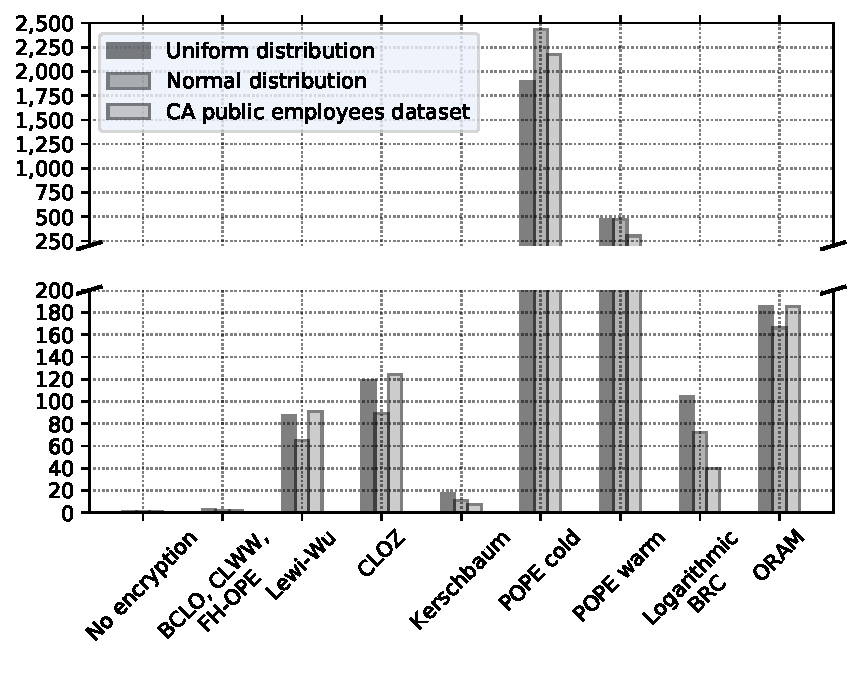
\includegraphics[width=1.0\textwidth]{protocol-charts-qios}
	\caption{Query stage number of I/O requests \cite[Figure 2d]{ore-benchmark-17}}\label{figure:ore}
\end{figure}

